\begin{figure}
	\begin{center}
	\scalebox{.7}{
		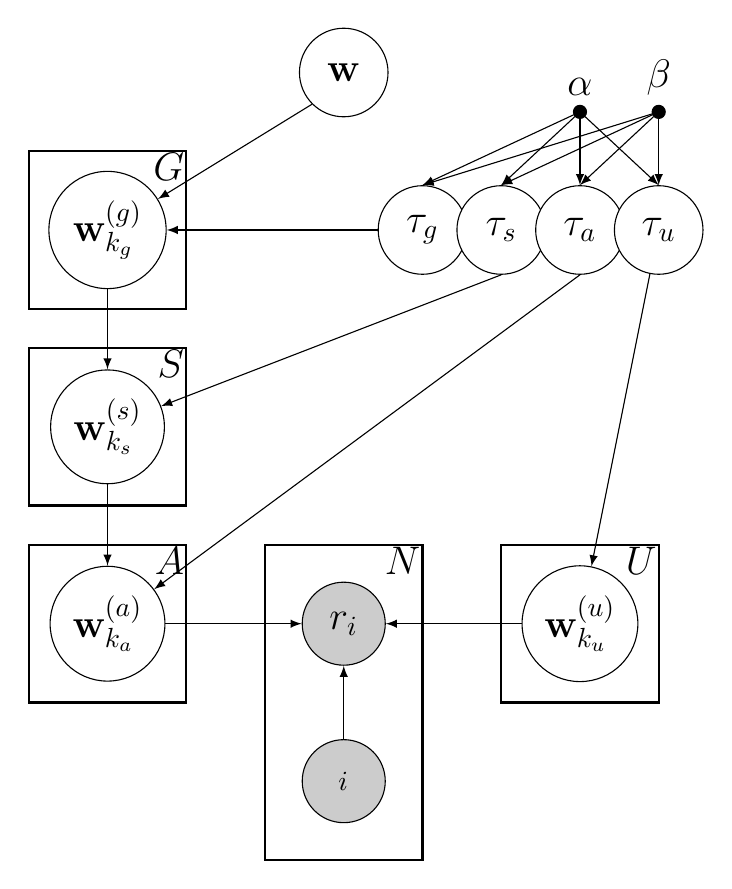
\begin{tikzpicture}[scale=1,,font=\Large,darkstyle/.style={circle,draw,fill=white!40,minimum size=32}]
		\tikzstyle{obsnode}=[circle,draw,fill=gray!40,minimum size=30]
		\tikzstyle{dot}=[circle,draw,fill=black,scale=0.5		]
		\tikzstyle{plate}=[draw,thick,minimum width=2cm,minimum height=2cm]
				\tikzstyle{plate2}=[draw,thick,minimum width=2cm,minimum height=4cm]
		\tikzstyle{line}=[draw]
		\tikzstyle{arrow}=[draw, -latex ]
		\tikzstyle{level 1}=[sibling distance=50mm]
		\tikzstyle{level 2}=[sibling distance=25mm]
		\tikzstyle{level 3}=[sibling distance=12mm]
		\tikzstyle{level 4}=[sibling distance=6mm]
		\tikzstyle{level 5}=[sibling distance=4mm,level distance=10mm]

\node[darkstyle](w) at(0,0){\textbf{w}} ;
\node[darkstyle](tg) at(1,-2){$\tau_g$} ;
\node[darkstyle](ts) at(2,-2){$\tau_s$} ;
\node[darkstyle](ta) at(3,-2){$\tau_a$} ;
\node[darkstyle](tu) at(4,-2){$\tau_u$} ;
\node[dot,label=above:{$\alpha$} ](alpha) at(3,-0.5){} ;
\node[dot,label=above:{$\beta$} ](beta) at(4,-0.5){} ;
\node[plate] (pg) at (-3,-2){} ;
		\node[darkstyle](g) at (-3,-2){$\textbf{w}^{(g)}_{k_g}$};
		\node[anchor=north east,inner sep=1pt] at (pg.north east){$G$};
		
		\node[plate] (ps) at (-3,-4.5){} ;
				\node[darkstyle](s) at (-3,-4.5){$\textbf{w}^{(s)}_{k_s}$};
		\node[anchor=north east,inner sep=1pt] at (ps.north east){$S$};
				\node[plate] (pa) at (-3,-7){} ;
				\node[darkstyle](a) at (-3,-7){$\textbf{w}^{(a)}_{k_a}$};
		\node[anchor=north east,inner sep=1pt] at (pa.north east){$A$};
					\node[plate] (pu) at (3,-7){} ;
		\node[darkstyle](u) at (3,-7){$\textbf{w}^{(u)}_{k_u}$};
		\node[anchor=north east,inner sep=1pt] at (pu.north east){$U$};
		
		\node[plate2] (p) at (0,-8){} ;
		\node[obsnode](r) at (0,-7){$r_{i}$};
		\node[obsnode](x) at (0,-9){$\x_{i}$};
		\node[anchor=north east,inner sep=1pt] at (p.north east){$N$};
\path[arrow]  (x) -- (r){};
\path[arrow]  (u) -- (r){};
\path[arrow]  (a) -- (r){};
\path[arrow]  (w.south west) -- (g){};
\path[arrow]  (g) -- (s){};
\path[arrow]  (s) -- (a){};
\path[arrow]  (ts.south) -- (s){};
\path[arrow]  (tg) -- (g){};
\path[arrow]  (ta.south) -- (a){};
\path[arrow]  (tu) -- (u){};
\path[arrow]  (alpha) -- (tu.north){};
\path[arrow]  (alpha) -- (ta.north){};
\path[arrow]  (alpha) --(tg.north){};
\path[arrow]  (alpha) -- (ts.north){};
\path[arrow]  (beta) -- (tu.north){};
\path[arrow]  (beta) -- (ta.north){};
\path[arrow]  (beta) -- (tg.north){};
\path[arrow]  (beta) -- (ts.north){};
	
	
		\end{tikzpicture}}
	%\vspace{-0.5cm}
	\end{center}
	\caption{A graphical model representation of the proposed model. Unshaded circles denote unobserved variables. Shaded circles denote observed variables. Solid dots denote hyper-parameters. }
	\label{fig:graphical_model}
\end{figure}